\documentclass{article}
\usepackage[T1]{fontenc}
\usepackage{lmodern}
\usepackage{graphicx}
\usepackage{amsmath,amssymb}
\usepackage[a4paper,margin=2cm]{geometry}
\usepackage[absolute,overlay]{textpos}
\setlength{\TPHorizModule}{1mm}
\setlength{\TPVertModule}{1mm}
\usepackage[indonesian]{babel}
\usepackage{hyperref}
\setlength{\emergencystretch}{2em}
% unit: Halaman 66

\begin{document}

% === Halaman 66 (llm) ===

\vspace{218.00mm}

\begin{center}
\large Mesin sandi di Museum Sandi Yogyakarta
\end{center}

% deskripsi: Foto sebuah mesin sandi berwarna abu-abu dengan papan ketik (keyboard) dan panel kontrol, bertuliskan SN-101.
% bbox normalisasi: [0.2420, 0.0920, 0.7990, 0.8260]
\begin{textblock*}{116.97mm}(50.82mm,27.32mm)
\noindent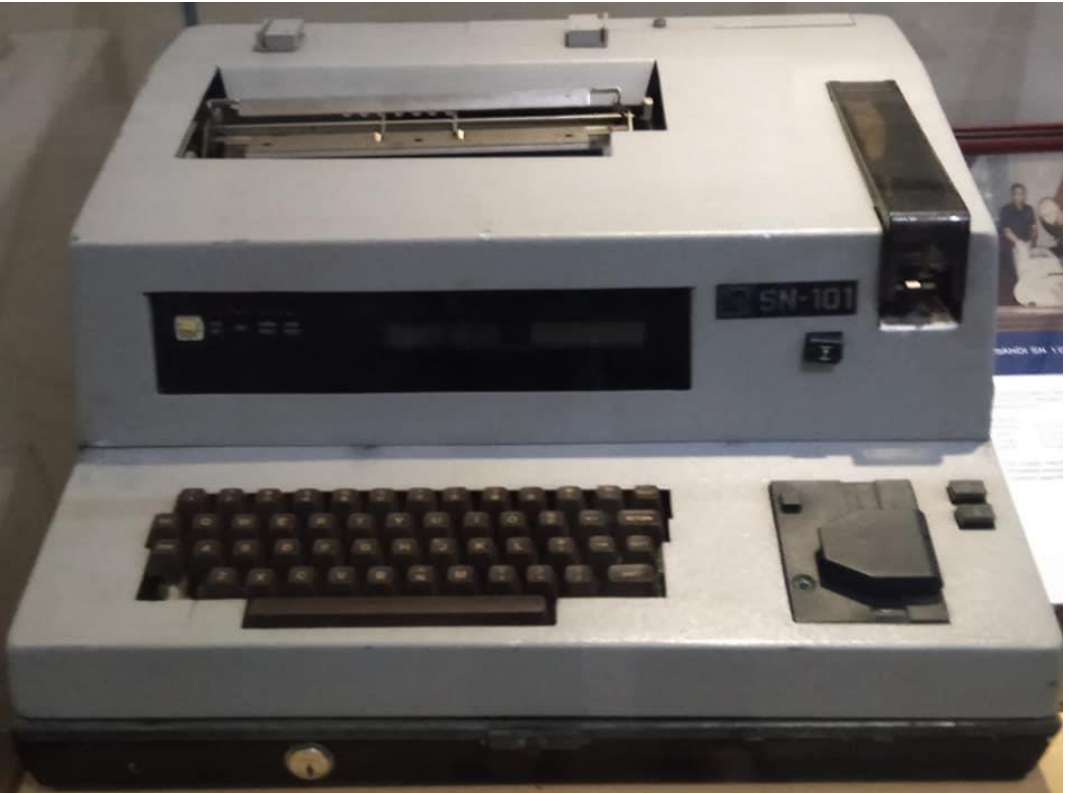
\includegraphics[width=116.97mm,height=218.00mm]{../../images/llm/page_066_img_01.png}%
\end{textblock*}

\end{document}
